%%%%%%%%%%%%%%%%%%%%%%%%%%%%%%%%%%%%%%%%%%%%%%%%%%%%%%%%%%%%%%%%%%%%%%%%%%%%%%%%
%2345678901234567890123456789012345678901234567890123456789012345678901234567890
%        1         2         3         4         5         6         7         8

\documentclass[letterpaper, 10 pt, conference]{ieeeconf}  % Comment this line out
                                                          % if you need a4paper
%\documentclass[a4paper, 10pt, conference]{ieeeconf}      % Use this line for a4
                                                          % paper

\IEEEoverridecommandlockouts                              % This command is only
                                                          % needed if you want to
                                                          % use the \thanks command
\overrideIEEEmargins
% See the \addtolength command later in the file to balance the column lengths
% on the last page of the document

\usepackage[utf8]{inputenc}
\usepackage[T1]{fontenc}
\usepackage{hyperref}
\usepackage{graphicx}
\usepackage{amsmath}
\usepackage{listings}
% The following packages can be found on http:\\www.ctan.org
%\usepackage{graphics} % for pdf, bitmapped graphics files
%\usepackage{epsfig} % for postscript graphics files
%\usepackage{mathptmx} % assumes new font selection scheme installed
%\usepackage{mathptmx} % assumes new font selection scheme installed
%\usepackage{amsmath} % assumes amsmath package installed
%\usepackage{amssymb}  % assumes amsmath package installed

\title{\LARGE \bf
\textit{Sample Sort}: Uma Análise Paralela Contraposta à Abordagem Sequencial}

%\author{ \parbox{3 in}{\centering Huibert Kwakernaak*
%         \thanks{*Use the $\backslash$thanks command to put information here}\\
%         Faculty of Electrical Engineering, Mathematics and Computer Science\\
%         University of Twente\\
%         7500 AE Enschede, The Netherlands\\
%         {\tt\small h.kwakernaak@autsubmit.com}}
%         \hspace*{ 0.5 in}
%         \parbox{3 in}{ \centering Pradeep Misra**
%         \thanks{**The footnote marks may be inserted manually}\\
%        Department of Electrical Engineering \\
%         Wright State University\\
%         Dayton, OH 45435, USA\\
%         {\tt\small pmisra@cs.wright.edu}}
%}

\author{Arthur Rodrigues Batista$^{1}$ e Douglas Ferreira Delefrati$^{2}$% <-this % stops a space
 \\Universidade Estadual de Maringá\\
   Departamento de informática\\
   Maringá, Paraná, Brasil
 \\ e-mail: ra105422@uem.br$^{1}$ | ra103654@uem.br$^{2}$
}


\begin{document}



\maketitle
\thispagestyle{empty}
\pagestyle{empty}


%%%%%%%%%%%%%%%%%%%%%%%%%%%%%%%%%%%%%%%%%%%%%%%%%%%%%%%%%%%%%%%%%%%%%%%%%%%%%%%%
\begin{abstract}
This work performs a quantitative analysis of the sequential and parallel performance of distributed memory of the sample sort  algorithm. Throughout the text, the operation of the sequential algorithm and which steps have been paralleled will be exposed. The results obtained were positive, reaching an increase of approximately 62\% in the final performance of the algorithm. The main limitations of the parallel version were the number of communications and synchronizations intrinsic to the algorithm, as well as the non-uniform distribution of elements in the buckets.

\end{abstract}

\begin{resumo}
Este trabalho realiza uma análise quantitativa do desempenho sequencial e paralelo de memória distribuída do algoritmo de ordenação \textit{sample sort}. Ao decorrer do texto, será exposto o funcionamento do algoritmo sequencial e quais as etapas que foram paralelizadas. Os resultados obtidos foram positivos, alcançando um aumento de aproximadamente $62\%$ no desempenho final do algoritmo. As principais limitações da versão paralela foi número de comunicações e sincronizações intrínsecas ao algoritmo, assim como a não uniformidade de distribuição de elementos nos \textit{buckets}.

\end{resumo}


%%%%%%%%%%%%%%%%%%%%%%%%%%%%%%%%%%%%%%%%%%%%%%%%%%%%%%%%%%%%%%%%%%%%%%%%%%%%%%%%
\section{Introdução}
A computação paralela é um tipo de computação na qual a execução de processos são realizados simultaneamente \cite{c5}. Existem diversas estratégias para paralelizar um código, neste trabalho exploramos a paralelização com um modelo de memória distribuída, sendo esse um paradigma fundamental para a computação paralela, especialmente para a programação numérica e científica \cite{c7}. 

No modelo de paralelização com memória distribuída, serão criados vários processos para a execução paralela, mas ao contrário do modelo de memória compartilhada, normalmente esses processos são executados em computadores distintos, comumente chamados de \textit{cluster}. Dessa forma, é possível usar o recurso computacional de mais de um servidor ao mesmo tempo \cite{c6}. As informações entre os processo são feitas através de troca de mensagens.
 
Para funcionar dessa forma o programa tem que ser explicitamente desenvolvido com essa capacidade. Geralmente isso é feito usando o protocolo de comunicação \textit{Message Passing Interface} (MPI). Esse protocolo fornece uma interface portátil simples, mas poderosa o suficiente para permitir que os programadores usem as operações de transmissão de mensagens de alto desempenho disponíveis em máquinas avançadas. Existem algumas implementações desse padrão e nesse trabalho utilizamos a implementação MPICH2.

Com o intuito de averiguar o desempenho do paralelismo, fora implementado duas versões do algoritmo de ordenação \textit{sample sort}, sendo uma versão sequencial e outra com o modelo de memória distribuída. Para tal, foram realizadas uma série de experimentos. Dentre estes, foi avaliado à performance à medida que o tamanho da entrada fosse variado, assim como a quantidade de processos. Ao decorrer do texto, elucidaremos em detalhes o funcionamentos do \textit{sample sort} e  como sua implementação paralela foi modelada.

Como citado anteriormente, o uso mais popular desse modelo de paralelização é utilizando \textit{clusters}. Entretanto, por limitações de \textit{hardware}, todos os testes foram realizados em uma máquina.

O resultado obtido fora um ganho médio de desempenho de $62\%$ e como esperado, o \textit{speed up} teve uma relação proporcional ao tamanho da entrada. O fator principal que obstruiu o \textit{speed up} ser próximo ao linear foi a grande quantidade de troca de mensagens e sincronização que são intrínsecas ao algoritmo. Sendo que uma vez desconsideradas as etapas de comunicação, o desempenho chegou a aumentar em até $82\%$.



\section{Trabalhos relacionados}
O \textit{sample sort} foi proposta em 1970 no trabalho \textit{amplesort: A Sampling Approach to Minimal Storage Tree Sorting} \cite{c11}. No qual os autores propõe uma modificação do \textit{quicksort} com uma ênfase no aprimoramento da complexidade de espaço. É possível observar que os artigos recentes estão focando em algoritmos eficientes para a memória cache baseados na estratégia de dividir e conquistar, pois com essa estratégia a paralelização desses problemas se tornam mais eficientes \cite{c2}. Os algoritmos mais conhecidos que se encaixam nessa descrição são o \textit{quicksort}, \textit{k-way merging} e \textit{radix sort}. 

Apesar do \textit{sample sort} ser um algoritmo conhecido, não é comum encontrar uma implementação apenas dele na literatura. Sendo mais habitual a utilização do algoritmo complementado com outras estratégias, como no trabalho \cite{c3} que fez uma mescla do \textit{simulated annealing}, \textit{sample sort} e busca tabu para um problema de agendamento distribuído, ou no trabalho \cite{c4} que utilizou a busca \textit{fuzzy}, \textit{simulated annealing} e \textit{sample sort} para abordar o mesmo problema.

\section{sample sort}

\subsection{Formulação do Problema}
O \textit{sample sort} é um algoritmo derivado do \textit{quicksort} que utiliza a estratégia de dividir e conquistar para decompor a entrada em partes menores e realizar o processamento em cada uma das partes individualmente. O principal problema de algoritmos que usam essa técnica é quando a distribuição do vetor não é uniforme, pois a granulação do código é comprometida e acaba por reduzir o desempenho. Diferentemente do \textit{quicksort}, no qual particiona a entrada em duas partes com base em um único valor chamado pivô, o \textit{sample sort} seleciona uma amostra de tamanho $S$ da sequência inicial e determina $p - 1$ elementos dessa amostra para ser os pivôs da ordenação. 

O algoritmo é composto pelas seguintes  fases:
\begin{enumerate}
    \item Dividir o vetor inicial em $n$ vetores uniformes.
    \item Escolha dos  $p - 1$ elementos uniformemente para serem os pivôs.
    \item Ordenar os $p - 1$ elementos e defina um \textit{bucket} para cada um.
    \item Posicionar cada elemento em seu respectivo \textbf{bucket}.
    \item Ordene cada \textit{bucket}.
\end{enumerate}

O pseudocódigo a seguir mostra o algoritmo supracitado mencionado.
\begin{lstlisting}[escapeinside={(*}{*)}]
sample sort(A[1..n], p, k)
    (*$S_p$*) = { (*$S_1,...,S_n$*) }
    select S = { (*$S_1,...,S_{(k-1)p}$*) }
    sort S
    {(*$S_0,...,S_p$*)} = {(*$-\infty,S_k,S_{2k},...,S_{(k-1)p}, \infty$*)}
    for each (*$a \in S_n$*)
        encontre (*$j$*) tal que (*$s_{j-1} < a \leq s_j$*)
        posicione (*$a$*) no bucket (*$b_j$*)
    for each (*$b \in b$*)
        sort b
    concatene cada bucket
        
    
\end{lstlisting}

Em detrimento da característica descentralizada do \textit{sample sort}, ele é conhecido por se um dos melhores algoritmos de ordenação para computadores paralelos com memória distribuída \cite{c2}. Na implementação do presente trabalho, as etapas 1, 4 e 5 foram executadas paralelamente. Na etapa 1 é realizado um operação de \textit{scatter} para distribuir o vetor inicial entre os processos. Em seguida, na etapa 2 é realizado operações de \textit{gather} para a escolha dos pivôs. Posteriormente, um processo ordena os $p - 1$ elementos de maneira sequencial e em seguida realiza um \textit{Broadcast} para que todos os processos saibam quais os \textit{buckets} escolhidos. Na próxima etapa cada processo realiza o posicionamentos dos seus elementos nos respectivos \textit{buckets}. Por fim, cada processo ordena os \textit{bukets} e envia para o processo raiz para realizar a concatenação. Sendo assim, o pseudocódigo pode ser escrito como

\begin{lstlisting}[escapeinside={(*}{*)}]
sample sort(A[1..n], p, k)
    (*$S_p$*) = MPI_Scatter({ (*$S_1,...,S_n$*) })
    select S = MPI_Gather({(*$S_1,...,S_{(k-1)p}$*)})
    sort S
    MPI_Broadcast(S)
    {(*$S_0,...,S_p$*)} = {(*$-\infty,S_k,S_{2k},...,S_{(k-1)p}, \infty$*)}
    for each (*$a \in S_n$*)
        encontre (*$j$*) tal que (*$s_{j-1} < a \leq s_j$*)
        posicione (*$a$*) no bucket (*$b_j$*)
    for each (*$b \in bukets$*)
        sort b
    MPI_SEND(b, ROOT)
    contatene cada bucket
\end{lstlisting}

\section{Metodologia}
Esta seção será dividida em duas subseções. Na primeira, adentraremos nas métricas que serão utilizadas a fim de avaliar o ganho de performance ao paralelizar o \textit{sample sort}. Em seguida, comentaremos a respeito das especificações técnicas da execução dos experimentos, tais como: a linguagem de programação e suas bibliotecas principais; máquina; quantidade de simulações e o tamanho dos dados de entradas.
\subsection{Métrica de Avaliação}
A principal métrica no âmbito de performance de processamento paralelo é o \textit{speed up} \cite{c10}, sendo definida como o tempo gasto serialmente para resolução de um problema dividido pelo tempo consumido para resolver o mesmo problema de maneira paralela em $p$ processos, como segue abaixo:
$$ S = \frac{T_{serial}}{T_{paralelo}}$$
Ao paralelizar um problema, o principal objetivo é atingir um \textit{speed up} dito linear, ou seja $S = p$, na qual cada processo realiza igualmente o mesmo trabalho que os demais. No entanto, sabe-se, por meio da litetura \cite{c10}, que atingir tal \textit{speed up} é dificilmente alcançável em detrimento sobretudo do custo necessário para realizar a comunicação entre os processos.

A segunda métrica adotada neste trabalho é a taxa de eficiência de \textit{speed up}, servindo como complemento à métrica original. Essa taxa mede o quão bem gasto está sendo o tempo para realização da tarefa entre os processos. Uma eficiência 100\% nos demonstra que cada processo está tendo a mesma performance que os demais.

Outra maneira de avaliarmos a performance da presente implementação é contrapôr com outras elaborações já conhecidas. Neste caso, utilizaremos os trabalhos do U-Coder \footnote{\url{https://www.ucoder.com.br/tutorials/sample_sort}} e Chang\footnote{\url{https://github.com/chunkaichang/MPI-sample-sort}} sujeitos aos mesmos experimentos do nossa implementação.


\subsection{Especificações dos Experimentos}

Essa seção descreve as especifidades do ambiente utilizado para executar os testes. Sendo que todos os experimentos foram realizados na linguagem de programação C. Ademais, para execução do código em paralelo, foi utilizado a biblioteca \textit{Message Passing Interface} (MPI).

\subsubsection{Máquina}
O experimento foi executado em uma máquina com um processador Intel i7-8550U (8) @ 4.000GHz, com quarto núcleos físicos e dois virtuais para cada. Além disso, a máquina também possui 8GB de memória principal. A versão do compilador de C utilizado neste trabalho é 10.2.0.
\subsubsection{Otimização e Quantidade de Simulações}
Para a compilação das duas abordagens foi utilizado a \textit{flag} de otimização O3. Ademais, os experimentos foram executados em 10 interações, utilizando os quarto núcleos físicos da máquina para obtenção de melhor performance.

\subsubsection{Entrada de Dados}
Os experimentos foram realizados utilizando três entradas distintas, representando o tamanho do arranjo na qual deseja-se ordenar, a Tabela 2 mostra essa relação:

{
\begin{table}[htbp]
\centering
\caption{Tamanho das entradas}
\begin{tabular}{lcc}
\hline
\textit{Nome} & \textit{Quantidade} \\ \hline
Pequena & 33554432 \\
Média & 67108864  \\
Grande & 134217728 \\ \hline
\end{tabular}
\label{table2}
\end{table}
}



\section{Resultados e Discussões}
A Figura 1 representa a taxa de \textit{speed up} pela quantidade de processos utilizados nos experimentos ao paralelizar as entradas pequena, média e grande. Já que a máquina na qual os experimentos foram realizados possui apenas 4 processadores, decidiu-se realizar toda discussão em torno da paralelização em 4 processos distintos. Isto posto, verifica-se inicialmente que ao passo que a entrada aumenta, há um aumento diretamente proporcional na taxa de \textit{speed up}. Na Figura 2, partindo da menor entrada para maior, houve uma melhoria de cerca de 13\%. Esse comportamento é esperado, haja vista que para implementação paralela do \textit{sample sort} a estratégia adotada fora paralelismo de dados, ou seja, distribui-se uma porção da sequência originalmente desordenada para cada processo e há uma série de operações realizadas por cada processo de forma que, ao unir suas saídas, tem-se um arranjo ordenado.
\begin{figure}[htbp]
      \centering
      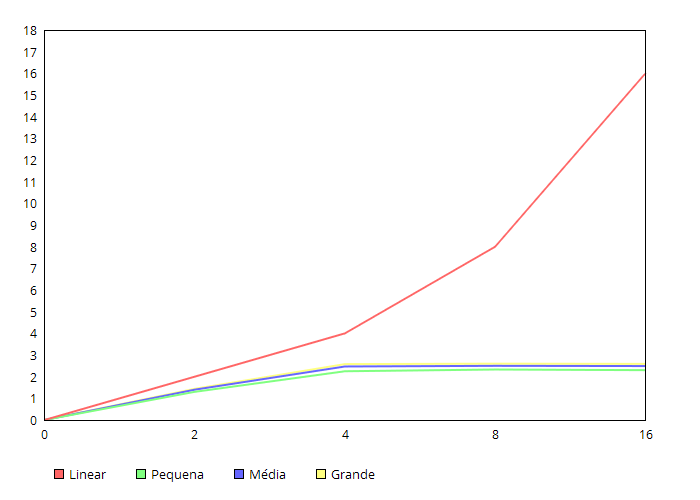
\includegraphics[scale=0.35]{speedup_multi.png}
      \caption{ Speed up em relação à quantidade de processos. Cada linha representa uma entrada diferente, com a vermelha sendo o speedup linear. }
      \label{figurelabel1}
\end{figure}

\begin{figure}[htbp]
      \centering
      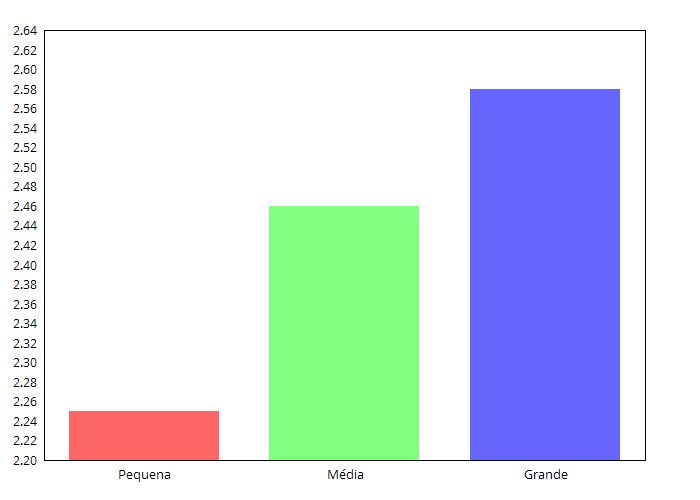
\includegraphics[scale=0.35]{four_pro.png}
      \caption{ Speed up em relação às entradas utilizando 4 processos. }
      \label{figurelabel2}
\end{figure}

No entanto, não houve uma taxa de eficiência 100\% de \textit{speed up} em relação aos experimentos realizados. Idealmente, espera-se que o \textit{speed up} seja igual ao número de processos na qual o problema fora distribuído (chamado \textit{speed up} linear), no presente cenário, sendo 4. A maior taxa de eficiência, entretanto, se considerarmos a maior entrada, foi de aproximadamente 63\%. 

No restante dessa seção, elencaremos algumas hipóteses para explicar tal resultado. A primeira explicação reside em um contexto empírico, sendo a investigação de implementações alternativas do \textit{sample sort}. Uma vez implementadas e sujeitas aos mesmos experimentos da presente proposta, contrapôs-se a taxa de \textit{speed up} as taxas de \textit{speed up} obtidas. A Figura 3 nos mostra esta comparação. Por meio da Figura, averiguarmos que além da nossa implementação possuir resultados melhores em relação à taxa de \textit{speed up}, nenhum das alternativas executadas conseguiram obter uma eficiência 100\%. 

\begin{figure}[htbp]
      \centering
      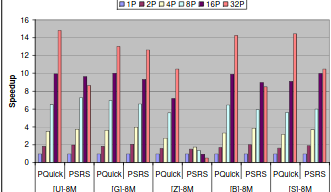
\includegraphics[scale=0.74]{trab_rela.png}
      \caption{Comparação ao paralelizar o sample sort (PSRS) e Quick Sort (PQuick), variando-se a quantidade de processos e com tamanho de entrada sendo 8000000 elementos \cite{c8}. }
      \label{figurelabel3}
\end{figure}

Para além desses resultados, foram investigados outros experimentos que visaram avaliar o desempenho ao paralelizar o \textit{sample sort} \cite{c8,c9}, nenhum alcançando 100 \% eficiência. A Figura 4 foi retirada de \cite{c8}, mediante a ela, verifica-se que a performance, em alguns casos, chega próximo ao ideal mas não o alcança. Em média, a eficiência, segundo os autores, constava entre 75\% até 95\% dependendo da técnica empregada.


\begin{figure}[htbp]
      \centering
      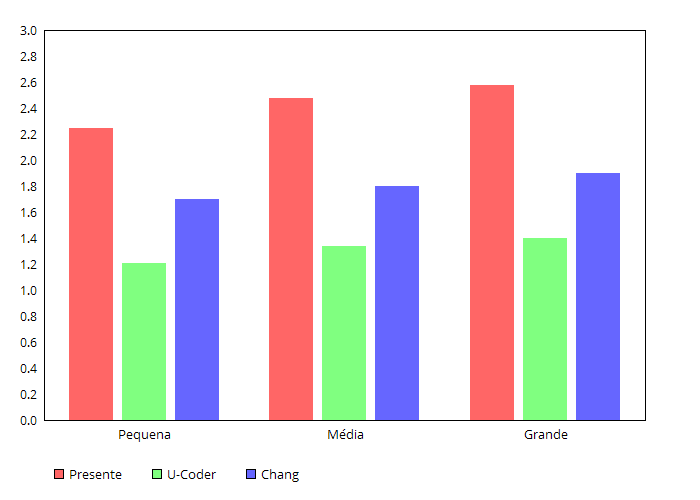
\includegraphics[scale=0.35]{comparison.png}
      \caption{ Speed up em relação ao tamanho da entrada utilizando 4 processos distribuídos. Cada cor corresponde à uma implementação distinta, sendo 'presente' deste trabalho. }
      \label{figurelabel4}
\end{figure}

Outra análise que faremos a seguir é em relação ao porquê dificilmente se chega a um \textit{speed up} linear no \textit{sample sort}. Primeiramente, sintetizamos às porcentagem de execução gasta pela paralelização do \textit{sample sort}, a Tabela 2 mostra esta relação, sendo dividida em três categorias, porcentagem gasta parar ordenar os elementos (ordenação); comunicação entre os processos (operações MPI) e outras instruções, como as chamadas de sistema, inicialização dos dados, etc. Nota-se que quase 25\% de todo processamento do programa está destinado à tratamento de comunicação entre os processos, se investirmos em maneiras mais otimizadas de trocar informações entre os processos, a taxa de \textit{speed up} teria um ganho significativo de performance. Com base nos experimentos realizados, se olharmos a Figura 5, é facilmente verificável que houve uma grande melhoria na taxa de \textit{speed up}, com a maior entrada tendo taxa de eficiência de 82\% se desconsiderarmos a comunicação entre os processos.

\begin{figure}[htbp]
      \centering
      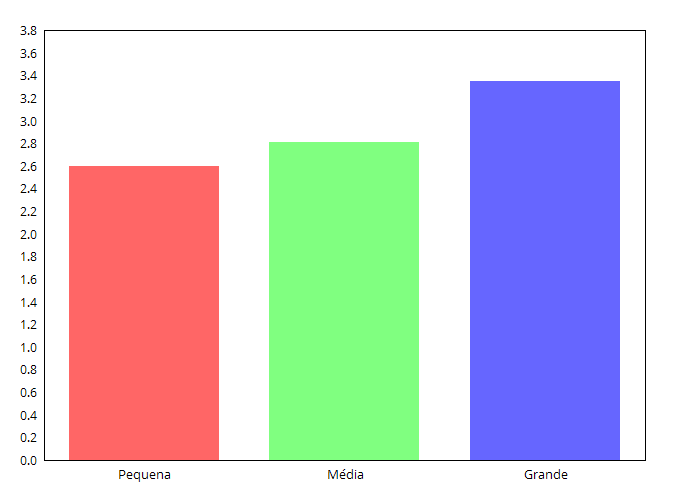
\includegraphics[scale=0.35]{sem_over.png}
      \caption{ Speed up em relação ao tamanho da entrada utilizando 4 processos distribuídos sem considerarmos o custo de comunicação entre os processos}
      \label{figurelabel5}
\end{figure}


{
\begin{table}[htbp]
\centering
\caption{Processamento da abordagem paralela}
\begin{tabular}{lcc}
\hline
\textit{Tipo} & \textit{Porcentagem} \\ \hline
Ordenação & 49.43\% \\
Operações MPI & 24.20\%  \\
Outros & 26.37\% \\ \hline
Total & 100\% \\ \hline
\end{tabular}
\label{table:db-segmentation-distribution}
\end{table}
}


\section{Conclusão}
Neste trabalho foi verificado os desafios de desenvolver um algoritmo utilizando paralelização com memória distribuída e quais as melhorias em relação ao desempenho esse modelo proporciona. Para tal, fora implementado duas versões do algoritmo de ordenação \textit{sample sort}, sendo uma versão sequencial e outra paralela. 

Como verificado ao longo do trabalho, o custo do \textit{overheading} teve um impacto significativo no desempenho, aproximadamente $13\%$ do tempo de execução. Para diminuir a quantidade de comunicação durante a execução do algoritmo, faz-se necessário a utilização de uma estrutura de árvore entre os processos \cite{c8}. Porém, em detrimento da complexidade de implementação dessa estrutura, foi optado por não utilizar a mesma.

Por fim, outro fator que impactou o desempenho da versão paralela foi a distribuição não uniforme dos elementos nos \textit{buckets}. Pois como essa etapa cada processo é atribuído um \textit{bucket} específico para ordenar e a concatenação dos resultados é utilizado no vetor final. Sendo assim, como a implementação utilizada do algoritmo não garante a uniformidade de elementos entre os processos, as instâncias que receberam uma quantidade menor de números para ordenar tem que esperar a instância com maior número finalizar. Para resolver essa adversidade, faz-se necessário a utilização das estruturas de árvores que foram supracitadas no texto. 

Portanto, para trabalhos futuros, pretende-se utilizar a estrutura descrita no trabalho \cite{c8} para averiguar as prováveis melhorias no desempenho do algoritmo, que segundo a literatura aproxima-se muito do \textit{speed up} linear.

\begin{thebibliography}{99}

\bibitem{c1} Peter Pacheco. 2011. An Introduction to Parallel Programming (1st. ed.). Morgan Kaufmann Publishers Inc., San Francisco, CA, USA.
\bibitem{c2} Sanders, Peter, and Sebastian Winkel. "Super scalar sample sort." European Symposium on Algorithms. Springer, Berlin, Heidelberg, 2004.
\bibitem{c3} Chan, Felix TS, et al. "A hybrid Tabu sample-sort simulated annealing approach for solving distributed scheduling problem." International Journal of Production Research 51.9 (2013): 2602-2619.
\bibitem{c4} Shukla, S.K., Son, Y.J. and Tiwari, M.K. Fuzzy based adaptive sample sort simulated annealing for resource-constrained project scheduling. Int J Adv Manuf Technol 36, 982–995 (2008). https://doi.org/10.1007/s00170-006-0907-6
\bibitem{c5}G. S. Almasi and A. Gottlieb. 1989. Highly parallel computing. Benjamin-Cummings Publishing Co., Inc., USA.
\bibitem{c6}Tanenbaum, Andrew S.; Steen, Maarten van (2002). Distributed systems: principles and paradigms. Upper Saddle River, NJ: Pearson Prentice Hall. 
\bibitem{c7}Callahan, David, and Ken Kennedy. "Compiling programs for distributed-memory multiprocessors." The Journal of Supercomputing 2.2 (1988): 151-169.
\bibitem{c8}Tsigas, P. and Y. Zhang. “Parallel Quicksort Seems to Outperform sample sort on Cache-coherent Shared Memory Multiprocessors : An Evaluation on SUN ENTERPRISE 10000.” (2002).
\bibitem{c9}H. Chen, S. Madaminov, M. Ferdman and P. Milder, "Sorting Large Data Sets with FPGA-Accelerated sample sort," 2019 IEEE 27th Annual International Symposium on Field-Programmable Custom Computing Machines (FCCM), San Diego, CA, USA, 2019, pp. 326-326, doi: 10.1109/FCCM.2019.00067.
\bibitem{c10}Peter Pacheco. 2011. An Introduction to Parallel Programming (1st. ed.). Morgan Kaufmann Publishers Inc., San Francisco, CA, USA.
\bibitem{c11}Frazer, W. D.; McKellar, A. C. (1970-07-01). "Samplesort: A Sampling Approach to Minimal Storage Tree Sorting". Journal of the ACM.
\end{thebibliography}





\end{document}
